% =================================================
% Faculty of Engineering, Zagazig University
% Computer and Systems Engineering Program
% CSE 2026 - IoT Laboratory
% Project: ESP8266 Lamp Control System
% =================================================

\documentclass[12pt,a4paper]{article}

% Packages
\usepackage[utf8]{inputenc}
\usepackage[T1]{fontenc}
\usepackage{geometry}
\usepackage{graphicx}
\usepackage{float}
\usepackage{booktabs}
\usepackage{array}
\usepackage{xcolor}
\usepackage{listings}
\usepackage{hyperref}
\usepackage{enumitem}
\usepackage{titlesec}
\usepackage{fancyhdr}
\usepackage{tikz}
\usetikzlibrary{arrows.meta, positioning, shapes.geometric}

% Page Setup
\geometry{
    top=2cm,
    bottom=2cm,
    left=2cm,
    right=2cm
}

% Hyperlinks
\hypersetup{
    colorlinks=true,
    linkcolor=black,
    urlcolor=blue,
    citecolor=black
}

% Header & Footer
\pagestyle{fancy}
\fancyhf{}

\lhead{CSE -- IoT Laboratory}
\rhead{ESP8266 Lamp Control System}
\cfoot{\thepage}

% Define programming languages
\lstdefinelanguage{JavaScript}{
    keywords={const, let, var, function, return, if, else, new,
              true, false, null, undefined, require, module},
    keywordstyle=\color{codeblue}\bfseries,
    ndkeywords={class, export, boolean, throw, implements, import},
    ndkeywordstyle=\color{codepurple}\bfseries,
    identifierstyle=\color{black},
    sensitive=true,
    comment=[l]{//},
    morecomment=[s]{/*}{*/},
    commentstyle=\color{codegreen}\itshape,
    stringstyle=\color{codepurple},
    morestring=[b]',
    morestring=[b]"
}

% Code Highlighting
\definecolor{codegreen}{RGB}{40,125,75}
\definecolor{codeblue}{RGB}{35,80,180}
\definecolor{codepurple}{RGB}{145,65,170}
\definecolor{codegray}{RGB}{110,110,110}
\definecolor{codebg}{RGB}{248,249,251}

\lstset{
    basicstyle=\ttfamily\footnotesize,
    backgroundcolor=\color{codebg},
    frame=single,
    rulecolor=\color{black!20},
    numbers=left,
    numberstyle=\tiny\color{codegray},
    numbersep=8pt,
    keywordstyle=\color{codeblue}\bfseries,
    commentstyle=\color{codegreen}\itshape,
    stringstyle=\color{codepurple},
    breaklines=true,
    breakatwhitespace=false,
    showstringspaces=false,
    keepspaces=true,
    tabsize=4,
    xleftmargin=1.5em,
    framexleftmargin=1.2em,
    aboveskip=0.8em,
    belowskip=0.8em,
    columns=fullflexible
}

% Document
\begin{document}

% Cover Page
\thispagestyle{empty}

\vspace{2cm}

\begin{center}
    {\large \textbf{Faculty of Engineering --- Zagazig University}}\\
    {\large Computer and Systems Engineering Program}\\[0.3cm]
    {\small CSE 2026: IOT Laboratory}

    \vspace{3cm}

    {\Huge \textbf{ESP8266 Lamp Control System}}
\end{center}

\vspace{4cm}

\begin{center}
    \renewcommand{\arraystretch}{1.5}
    \begin{tabular}{|p{5cm}|p{3cm}|p{3cm}|}
        \hline
        \textbf{Name}    & \textbf{Section} & \textbf{Nummber} \\
        \hline
        Youssef Reda     & 2                & 30               \\
        \hline
        Mohamed Moustafa & 2                & 16               \\
        \hline
        Osamn Mohamed    & 1                & 24               \\
        \hline
    \end{tabular}
\end{center}

\vfill

\begin{center}
    Academic Year 2026/2027
\end{center}

\newpage

% Table of Contents
\tableofcontents

% 1. Introduction

\newpage
\section*{Introduction}

\vspace{0.3cm}

\subsection*{Project Overview}
This project presents an IoT-based lamp control system using an ESP8266
microcontroller and a web-based dashboard. The system enables users to
control the built-in LED remotely through a WebSocket connection, allowing
real-time updates to the lamp state and brightness.

\vspace{0.5cm}

\subsection*{Problem Statement}
Controlling an electronic device directly through physical interaction
limits the flexibility of remote operation. This project addresses this
limitation by providing a web interface that communicates with an ESP8266
over Wi-Fi through a Node.js backend, enabling remote lamp control within
the connected network.

\vspace{0.5cm}

\subsection*{Project Objectives}
The main objectives of this project are to:
\begin{itemize}
    \item Establish Wi-Fi connectivity between the ESP8266 and the system.
    \item Develop a web dashboard for lamp control and brightness adjustment.
    \item Implement WebSocket communication for exchanging commands and state updates.
    \item Synchronize the displayed lamp state with the backend state.
\end{itemize}

\addcontentsline{toc}{section}{Introduction}
\addcontentsline{toc}{subsection}{Project Overview}
\addcontentsline{toc}{subsection}{Problem Statement}
\addcontentsline{toc}{subsection}{Project Objectives}

% 2. System Requirements and Technologies

\newpage
\section*{System Requirements and Technologies}

\vspace{0.2cm}

\subsection*{Hardware Components}
\begin{itemize}
    \item ESP8266 development board with a built-in LED.
    \item Computer for running the Node.js backend and accessing the web dashboard.
    \item Wi-Fi network for communication between the ESP8266 and the backend.
\end{itemize}

\vspace{0.5cm}

\subsection*{Software and Development Tools}
\begin{itemize}
    \item Node.js runtime environment.
    \item Web browser for accessing the control dashboard.
    \item Arduino IDE for developing and uploading the ESP8266 firmware.
    \item Code editor for developing the backend and frontend.
\end{itemize}

\vspace{0.5cm}

\subsection*{Technologies and Libraries}
\begin{itemize}
    \item \textbf{Express.js:} Serves the dashboard and handles HTTP routes.
    \item \textbf{ws:} Provides WebSocket communication on the Node.js server.
    \item \textbf{WebSockets:} Enables bidirectional communication between the dashboard, backend, and connected device.
    \item \textbf{ArduinoJson:} Parses JSON messages received by the ESP8266.
    \item \textbf{ESP8266WiFi:} Connects the microcontroller to the Wi-Fi network.
    \item \textbf{WebSocketsClient\_Generic:} Provides WebSocket client functionality on the ESP8266.
    \item \textbf{HTML, CSS, and JavaScript:} Build the web dashboard and its interactive controls.
\end{itemize}

\addcontentsline{toc}{section}{System Requirements and Technologies}
\addcontentsline{toc}{subsection}{Hardware Components}
\addcontentsline{toc}{subsection}{Software and Development Tools}
\addcontentsline{toc}{subsection}{Technologies and Libraries}

% 3. System Design and Architecture

\newpage
\section*{System Design and Architecture}

\vspace{0.2cm}

\subsection*{Overall System Architecture}

The system consists of a web dashboard, a Node.js backend,
an ESP8266 microcontroller, and a built-in LED. The dashboard
communicates with the backend through WebSockets. The backend
maintains the lamp state and broadcasts state updates to all
connected WebSocket clients, including the dashboard and ESP8266.
The microcontroller processes the received state and controls
the LED output accordingly.

\begin{figure}[htbp]
    \centering
    \resizebox{\textwidth}{!}{%
        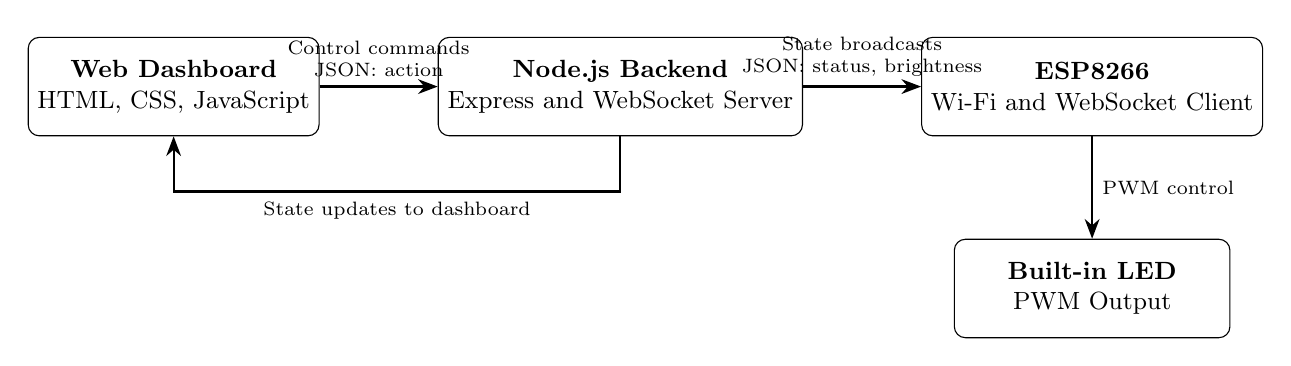
\begin{tikzpicture}[
                node distance=1.5cm,
                component/.style={
                        draw,
                        rounded corners,
                        minimum width=3.5cm,
                        minimum height=1.25cm,
                        align=center,
                        font=\small
                    },
                connection/.style={
                        -{Stealth[length=2.5mm]},
                        thick
                    },
                bidirectional/.style={
                        {Stealth[length=2.5mm]}-{Stealth[length=2.5mm]},
                        thick
                    }
            ]

            \node[component] (dashboard) {
                \textbf{Web Dashboard}\\
                HTML, CSS, JavaScript
            };

            \node[component, right=of dashboard] (backend) {
                \textbf{Node.js Backend}\\
                Express and WebSocket Server
            };

            \node[component, right=of backend] (esp) {
                \textbf{ESP8266}\\
                Wi-Fi and WebSocket Client
            };

            \node[component, below=1.3cm of esp] (led) {
                \textbf{Built-in LED}\\
                PWM Output
            };

            \draw[connection]
            (dashboard) -- node[above, align=center, font=\scriptsize]
            {Control commands\\JSON: action}
            (backend);

            \draw[connection]
            (backend) -- node[above, align=center, font=\scriptsize]
            {State broadcasts\\JSON: status, brightness}
            (esp);

            \draw[connection]
            (esp) -- node[right, font=\scriptsize]
            {PWM control}
            (led);

            \draw[connection]
            (backend.south) -- ++(0,-0.7)
            -| node[pos=0.25, below, font=\scriptsize]
                {State updates to dashboard}
            (dashboard.south);

        \end{tikzpicture}%
    }
    \caption{Overall architecture of the ESP8266 lamp control system.}
    \label{fig:system-architecture}
\end{figure}

\vspace{0.5cm}

\subsection*{System Components and Responsibilities}

The web dashboard provides controls for switching the lamp on
and off and adjusting its brightness. The Node.js backend
processes incoming commands and maintains the lamp state in
memory through the lamp service. The WebSocket server
broadcasts the updated state to connected clients. The ESP8266
receives these updates and applies the corresponding output
to its built-in LED.

\vspace{0.8cm}

\subsection*{Communication Protocol and Message Format}

WebSocket communication is used to exchange messages between
the dashboard and the backend and to deliver state updates to
the connected ESP8266. Messages are encoded in JSON format.

The dashboard sends commands containing an \texttt{action}
field, such as \texttt{on}, \texttt{off}, or
\texttt{change\_brightness}, with a brightness value when
applicable. After processing a command, the backend broadcasts
a state object containing the \texttt{status} and
\texttt{brightness} fields. The ESP8266 uses these fields to
determine the required LED output.

\newpage
\subsection*{System Workflow and Data Flow}

When a user interacts with the dashboard, the browser sends
a command to the backend. The backend updates the in-memory
lamp state and broadcasts the resulting state to all connected
WebSocket clients. The dashboard updates its interface, while
the ESP8266 processes the broadcast and adjusts the LED output.

\vspace{0.8cm}

\begin{figure}[htbp]
    \centering
    \resizebox{\textwidth}{!}{%
        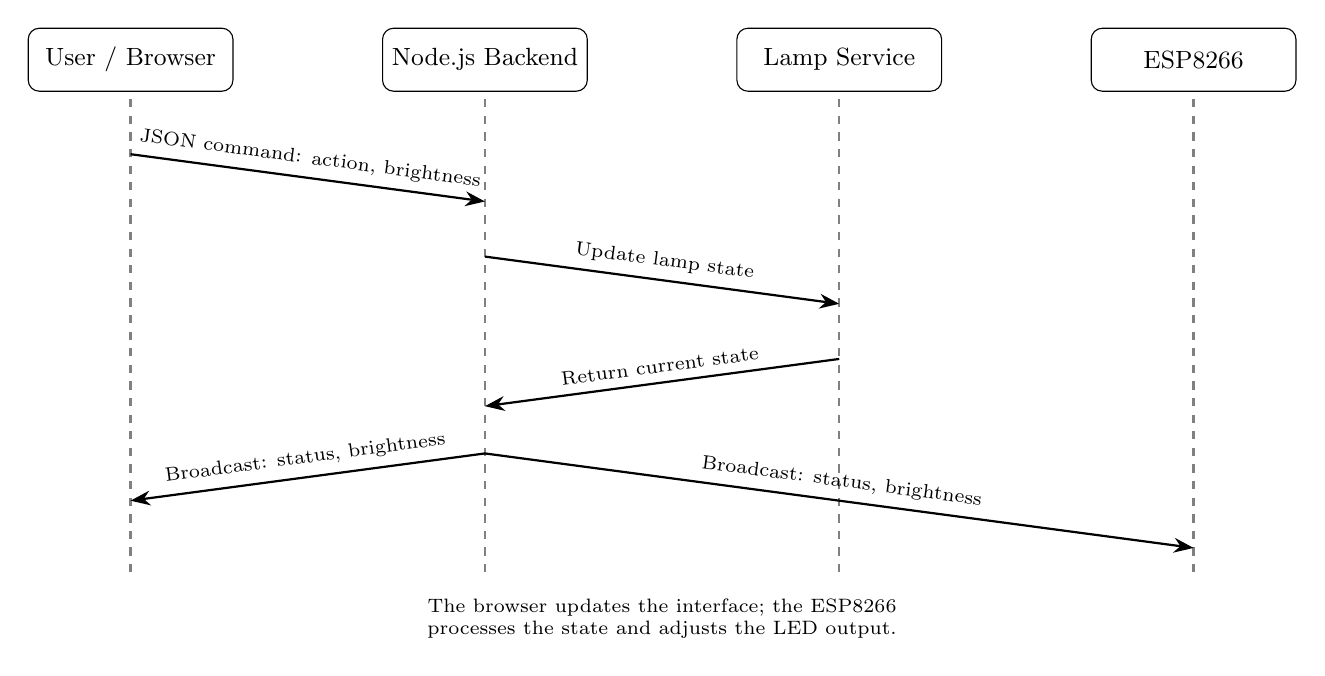
\begin{tikzpicture}[
                actor/.style={
                        draw,
                        rounded corners,
                        minimum width=2.6cm,
                        minimum height=0.8cm,
                        align=center,
                        font=\small
                    },
                lifeline/.style={
                        dashed,
                        gray,
                        thick
                    },
                message/.style={
                        -{Stealth[length=2.5mm]},
                        thick
                    }
            ]

            \node[actor] (user) at (0,0) {User / Browser};
            \node[actor] (server) at (4.5,0) {Node.js Backend};
            \node[actor] (service) at (9,0) {Lamp Service};
            \node[actor] (esp) at (13.5,0) {ESP8266};

            \foreach \x in {0,4.5,9,13.5} {
                    \draw[lifeline] (\x,-0.5) -- (\x,-6.5);
                }

            \draw[message] (0,-1.2) -- node[above, sloped, font=\scriptsize]
            {JSON command: action, brightness} (4.5,-1.8);

            \draw[message] (4.5,-2.5) -- node[above, sloped, font=\scriptsize]
            {Update lamp state} (9,-3.1);

            \draw[message] (9,-3.8) -- node[above, sloped, font=\scriptsize]
            {Return current state} (4.5,-4.4);

            \draw[message] (4.5,-5.0) -- node[above, sloped, font=\scriptsize]
            {Broadcast: status, brightness} (0,-5.6);

            \draw[message] (4.5,-5.0) -- node[above, sloped, font=\scriptsize]
            {Broadcast: status, brightness} (13.5,-6.2);

            \node[align=center, font=\scriptsize] at (6.75,-7.1)
            {The browser updates the interface; the ESP8266\\
                processes the state and adjusts the LED output.};

        \end{tikzpicture}%
    }
    \caption{Sequence of a lamp control command and state broadcast.}
    \label{fig:communication-sequence}
\end{figure}

\addcontentsline{toc}{section}{System Design and Architecture}
\addcontentsline{toc}{subsection}{Overall System Architecture}
\addcontentsline{toc}{subsection}{System Components and Responsibilities}
\addcontentsline{toc}{subsection}{Communication Protocol and Message Format}
\addcontentsline{toc}{subsection}{System Workflow and Data Flow}

% 4. System Implementation

\newpage
\section*{System Implementation}

\vspace{0.2cm}

\subsection*{Backend Implementation}

The Node.js backend uses Express.js to serve the dashboard
and handle HTTP requests. A WebSocket server runs on port
2000, while a dedicated lamp service maintains the current
lamp status and brightness in memory.

\vspace{1cm}

\begin{lstlisting}[
    language=JavaScript,
    caption={HTTP and WebSocket Server Initialization},
    label={lst:server-init}
]
const app = require('./server/server.js');
const http = require('node:http');
const createWebSocketServer = require('./websocket/websocket.js');

const server = http.createServer(app);
createWebSocketServer(server);

const PORT = 2000;

server.listen(PORT, () => {
    console.log(`Server is running at port ${PORT}`);
});
\end{lstlisting}

\vspace{1cm}

\begin{lstlisting}[
    language=JavaScript,
    caption={Express.js Application and HTTP Route Configuration},
    label={lst:app-routes}
]
const express = require('express');
const app = express();
const path = require('node:path')

app.use(express.static(path.join(__dirname, '..', 'views')));

app.get('/', (req, res) => {
    res.sendFile(path.join(__dirname, '..', 'views', 'index.html'));
});

// Testing endpoint

app.get('/api/test', (req, res) => {
    res.json({
        status: 'ok',
        message: "Backend is runnig"
    });
});

module.exports = app;
\end{lstlisting}

\newpage
\subsection*{Web Dashboard Implementation}

The dashboard is built with HTML, CSS, and JavaScript.
It provides power and brightness controls, displays the
connection status, and sends JSON commands to the backend
through WebSockets.

\vspace{1cm}

\begin{lstlisting}[
    language=JavaScript,
    caption={Web Dashboard Controls and WebSocket Communication},
    label={lst:dashboard-control}
]
const HOST = location.origin.replace(/^http/, 'ws');
const ws = new WebSocket(HOST);

.....

ws.onopen = function () {
    console.log("Connected to WebSocket server");
    setConnectionConnected();
    turnLampOn(255);
};

powerBtn.onclick = () => {
    if (isOn) {
        turnLampOff();
    } else {
        turnLampOn(255);
    }
};

slider.addEventListener('input', () => {
    brightnessVal.textContent = slider.value;
});

slider.addEventListener('change', () => {
    const brightness = Number(slider.value);

    if (brightness === 0) {
        turnLampOff();
    } else {
        setLampOnUI(brightness);

        lampCommand['action'] = "change_brightness";
        lampCommand['brightness'] = brightness;
        if (ws.readyState === WebSocket.OPEN) {
            ws.send(JSON.stringify(lampCommand));
        }
    }
});

ws.onmessage = function (event) {
    let lampStatus = JSON.parse(event.data);

    if (lampStatus.status === "on") {
        brightness = lampStatus.brightness;
        setLampOnUI(brightness);
    } else if (lampStatus.status === "off") {
        setLampOffUI();
    }
};

ws.onerror = function () {
    setConnectionDisconnected();
};

ws.onclose = function () {
    console.log("WebSocket connection closed");
    setConnectionDisconnected();
    setLampOffUI();
};
\end{lstlisting}

\vspace{0.5cm}

\subsection*{ESP8266 Firmware Implementation}

The ESP8266 firmware uses the Wi-Fi, WebSocket client,
and ArduinoJson libraries. It connects to the configured
Wi-Fi network, receives JSON state messages, and controls
the built-in LED. A five-second WebSocket reconnection
interval is configured.

\vspace{1cm}

\begin{lstlisting}[
    language=C++,
    caption={ESP8266 LED Control and PWM Implementation},
    label={lst:esp8266-control}
]
#include <ESP8266WiFi.h>
#include <WebSocketsClient_Generic.h>
#include <ArduinoJson.h>

// Configurations
constexpr char WIFI_SSID[] = "SSID";
constexpr char WIFI_PASSWORD[] = "PASSWORD";

constexpr char SERVER[] = "SERVER_ADDRESS";
constexpr uint16_t SERVER_PORT = 2000;
constexpr char SERVER_PATH[] = "/";

constexpr uint8_t LED_PIN = LED_BUILTIN;

// WebSocket
WebSocketsClient webSocket;

// Command execution
void executeCommand(JsonDocument &json)
{
    const char *status = json["status"];
    int brightness = json["brightness"] | 0;

    if (status == nullptr)
    {
        Serial.println("Warning: Received JSON without a 'status' field.");
        return;
    }

    Serial.print("Executing status: ");
    Serial.print(status);
    Serial.print(" | brightness: ");
    Serial.println(brightness);

    if (strcmp(status, "on") == 0)
    {
        // LED_BUILTIN is usually active-low on ESP8266, so 255 - brightness works perfectly
        analogWrite(LED_PIN, 255 - brightness);
        Serial.println("LED updated (ON)");
    }
    else if (strcmp(status, "off") == 0)
    {
        analogWrite(LED_PIN, 255);
        Serial.println("LED turned OFF");
    }
}

// JSON message
void handleMessage(uint8_t *payload, size_t length)
{
    Serial.print("Received raw payload: ");
    for (size_t i = 0; i < length; i++)
    {
        Serial.print((char)payload[i]);
    }
    Serial.println();

    JsonDocument json;

    DeserializationError error =
        deserializeJson(json, payload, length);

    if (error)
    {
        Serial.print("Invalid JSON: ");
        Serial.println(error.c_str());
        return;
    }

    executeCommand(json);
}

// WebSocket events
void onWebSocketEvent(
    WStype_t type,
    uint8_t *payload,
    size_t length)
{
    switch (type)
    {
    case WStype_CONNECTED:
        Serial.print("[WSc] Connected to url: ");
        Serial.println((char *)payload);
        break;

    case WStype_DISCONNECTED:
        Serial.println("[WSc] Disconnected from server.");
        break;

    case WStype_TEXT:
        Serial.println("[WSc] Received TEXT message.");
        handleMessage(payload, length);
        break;

    case WStype_ERROR:
        Serial.println("[WSc] Error occurred!");
        break;

    default:
        Serial.print("[WSc] Unhandled event type: ");
        Serial.println(type);
        break;
    }
}

void setup()
{
    Serial.begin(921600);

    pinMode(LED_PIN, OUTPUT);

    // LED off
    analogWrite(LED_PIN, 255);

    // Wi-Fi
    WiFi.begin(WIFI_SSID, WIFI_PASSWORD);

    Serial.print("Connecting to Wi-Fi");

    while (WiFi.status() != WL_CONNECTED)
    {
        delay(250);
        Serial.print(".");
    }

    Serial.println();

    Serial.print("Wi-Fi connected. IP: ");
    Serial.println(WiFi.localIP());

    // WebSocket
    webSocket.begin(
        SERVER,
        SERVER_PORT,
        SERVER_PATH);

    webSocket.onEvent(onWebSocketEvent);
    webSocket.setReconnectInterval(5000);

    Serial.println("WebSocket client started.");
}

void loop()
{
    webSocket.loop();
}
\end{lstlisting}

\newpage
\subsection*{Lamp State and Brightness Control}

The backend stores the lamp status and brightness, using
values from 0 to 255. Turning the lamp on sets the brightness
to 255, while turning it off sets it to zero. The ESP8266
uses \texttt{analogWrite()} and an active-low PWM mapping
to control the built-in LED.

\vspace{1cm}

\begin{lstlisting}[
    language=JavaScript,
    caption={Lamp State Management and Control Functions},
    label={lst:lamp-service}
]
const lamp = {
    status: "off",
    brightness: 0
};

function turnOn() {
    lamp.status = "on";
    lamp.brightness = 255;
};

function turnOff() {
    lamp.status = "off";
    lamp.brightness = 0;
};

function setBrightness(value) {
    lamp.status = "on";
    lamp.brightness = value;
};

function getStatus() {
    return lamp;
};

module.exports = {
    turnOn,
    turnOff,
    setBrightness,
    getStatus
};
\end{lstlisting}

\newpage
\subsection*{WebSocket Communication and Synchronization}

The dashboard sends commands using the \texttt{action}
field. The backend updates the lamp state and broadcasts
\texttt{status} and \texttt{brightness} to connected clients.
The dashboard updates its interface, and the ESP8266
adjusts the LED output based on the received state. The
backend does not receive explicit confirmation of the
physical LED state.

\vspace{1cm}

\begin{lstlisting}[
    language=JavaScript,
    caption={WebSocket Message Handling and State Broadcasting},
    label={lst:websocket-handler}
]
const lampService = require('../services/lampService.js');
const SocketServer = require('ws').Server;

function createWebSocketServer(server) {
    const wss = new SocketServer({ server });

    wss.on("connection", (ws) => {
        console.log('Client connected');

        ws.on('message', (msg) => {
            const lampStatus = msg.toString();
            const lampCommand = JSON.parse(lampStatus);

            if (lampCommand.action === "on") {
                lampService.turnOn();
            } else if (lampCommand.action === "off") {
                lampService.turnOff();
            } else if (lampCommand.action === "change_brightness") {
                lampService.setBrightness(lampCommand.brightness);
            }

            const lampState = lampService.getStatus();

            broadcast(wss, lampState);

            console.log("Message form client: ", lampStatus);
        });

        ws.on('close', () => {
            console.log('Client disconnected');
        });
    });

    return wss;
};

function broadcast(wss, lampState) {
    const message = JSON.stringify(lampState);

    wss.clients.forEach(function (client) {
        if (client.readyState === client.OPEN) {
            client.send(message);
        } else {
            console.log("Clinet off");
        }
    });
}

module.exports = createWebSocketServer;
\end{lstlisting}

\addcontentsline{toc}{section}{System Implementation}
\addcontentsline{toc}{subsection}{Backend Implementation}
\addcontentsline{toc}{subsection}{Web Dashboard Implementation}
\addcontentsline{toc}{subsection}{ESP8266 Firmware Implementation}
\addcontentsline{toc}{subsection}{Lamp State and Brightness Control}
\addcontentsline{toc}{subsection}{WebSocket Communication and Synchronization}

% 5.Testing and Results

\newpage
\section*{Testing and Results}

The system was evaluated by checking the interaction between
the web dashboard, the Node.js backend, and the ESP8266
controller. The main operations considered were establishing
the WebSocket connection, switching the lamp on and off,
adjusting brightness, and updating the displayed lamp state.
Screenshots of the implemented system and its observed
behavior are provided below to document the testing process.

\vspace{1cm}

\begin{figure}[H]
    \centering
    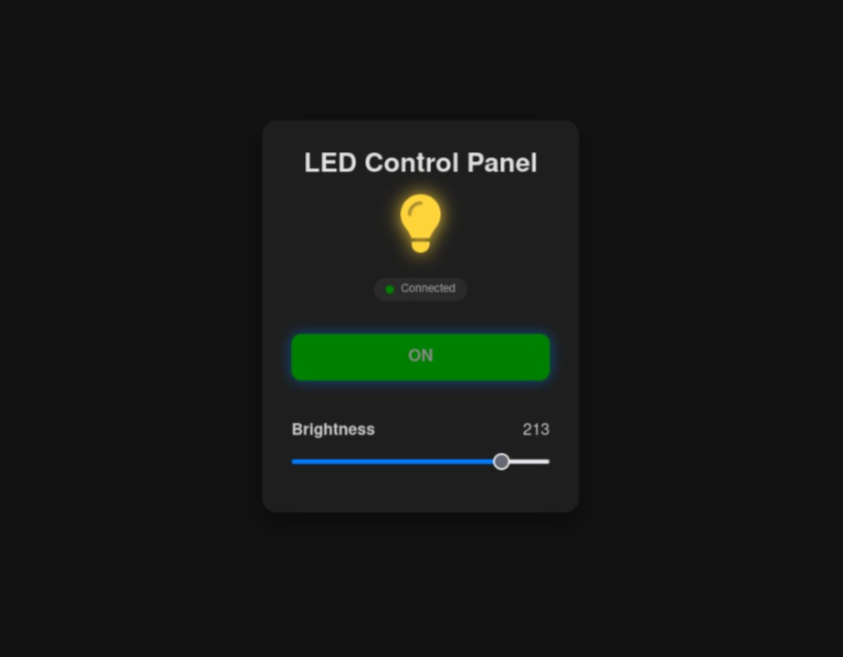
\includegraphics[width=0.85\textwidth]
    {../assets/dashboard.png}
    \caption{Web Dashboard Interface}
    \label{fig:dashboard}
\end{figure}

\vspace{0.5cm}

\begin{figure}[H]
    \centering
    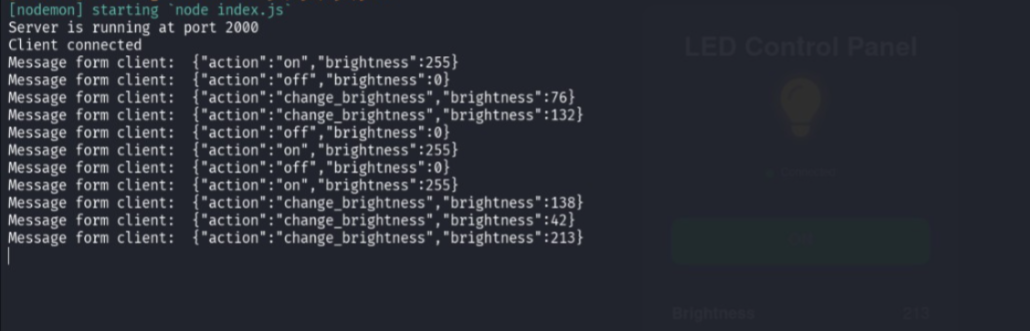
\includegraphics[width=0.85\textwidth]
    {../assets/websocket_connection.png}
    \caption{WebSockets connection}
    \label{fig:dashboard}
\end{figure}

\begin{figure}[H]
    \centering
    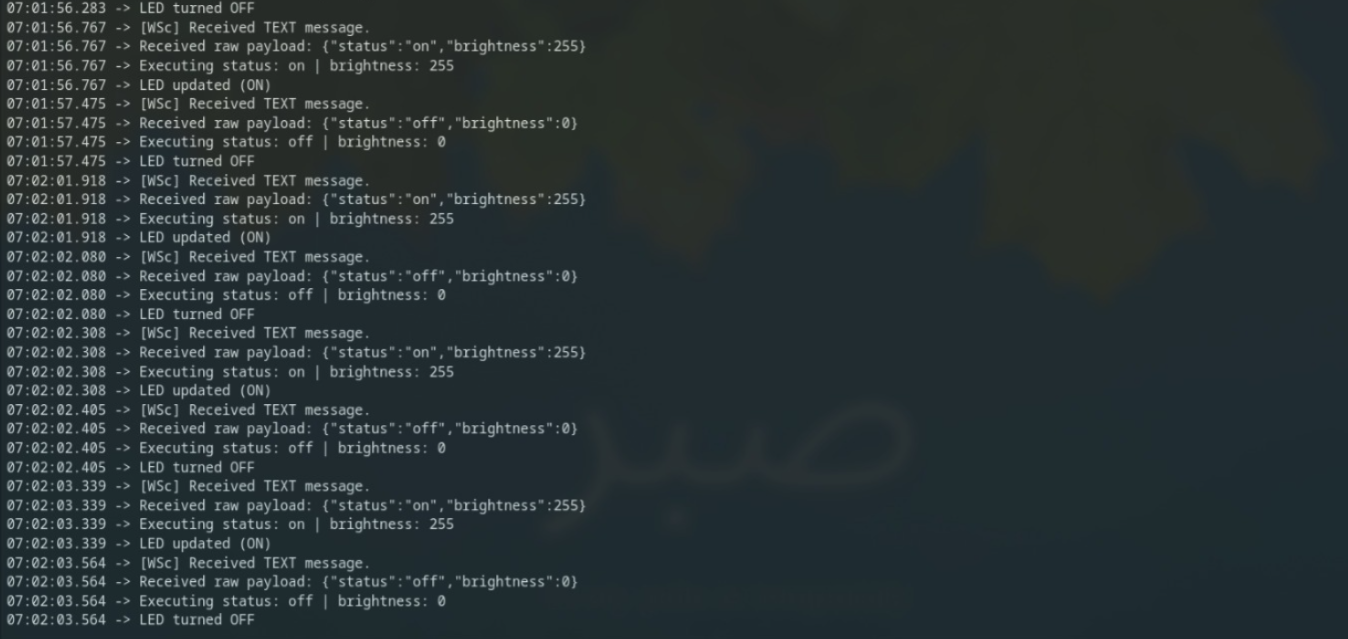
\includegraphics[width=0.85\textwidth]
    {../assets/esp_received_messages.png}
    \caption{ESP8266 Serial Monitor Output During WebSocket Communication}
    \label{fig:esp-serial-monitor}
\end{figure}

\addcontentsline{toc}{section}{Testing and Results}

% References

\newpage
\phantomsection
\addcontentsline{toc}{section}{References}

\begin{thebibliography}{9}

    \bibitem{project-repo}
    Youssef.Reda, \textit{CSE3-IOT-Labs: IoT Laboratory Projects}.
    GitHub Repository.
    Available at:
    \url{https://github.com/Youssef-Reda440/CSE3-IOT-Labs}

    \bibitem{iot-playlist}
    IoT Laboratory Teaching Assistant,
    \textit{IoT Laboratory Tutorials}.
    YouTube Playlist.
    Available at:
    \url{https://youtube.com/playlist?list=PLKrTtHfjR9toHOJ1ZnHn-700OwPN-eG_N}

\end{thebibliography}

\end{document}